\documentclass{jarticle}
\usepackage[dvipdfmx]{graphicx}
\usepackage{here}
\usepackage{listings,jlisting}


\lstset{
  basicstyle={\ttfamily},
  identifierstyle={\small},
  commentstyle={\smallitshape},
  keywordstyle={\small\bfseries},
  ndkeywordstyle={\small},
  stringstyle={\small\ttfamily},
  frame={tb},
  breaklines=true,
  columns=[l]{fullflexible},
  numbers=left,
  xrightmargin=0zw,
  xleftmargin=3zw,
  numberstyle={\scriptsize},
  stepnumber=1,
  numbersep=1zw,
  lineskip=-0.5ex
}

\title{{システム実験}\\基礎実験4レポート}
\author{6119019056 山口力也}
\date{2019/05/17日提出}

\begin{document}
\maketitle
\section{基礎実験第4回の概要}
基礎実験第4回目の実験の目的,実施した実験の概要,および理解した事柄を100~200字程度で説明せよ.

\subsection{実験目的}
以下の示す事柄を実験目的とした.

\begin{itemize}

\item 割り込みの動作原理を知る.
\item ポーリングと割り込みの処理の違いを理解する.
\item タイマ割り込みの動作原理を理解して使いこなせる.
\item 外部割り込みの動作原理を理解して使いこなせる.

\end{itemize}

\subsection{実験概要}
実験内容としてマイコンを用いた割り込み処理として"タイマ割り込み"と"外部割り込み"を扱った.

\subsection{理解した事柄}
マイコンのプログラムをより効率的に実行する割り込み機能の動作原理を理解し,実装方法を習得し理解した.

\section{回路実装}
基礎実験4で使用した回路のブレッドボード配線図を報告せよ.

以下\ref{fig:bread}に使用した回路のブレッドボード配線図を示す.

\begin{figure}[H]
\begin{center}
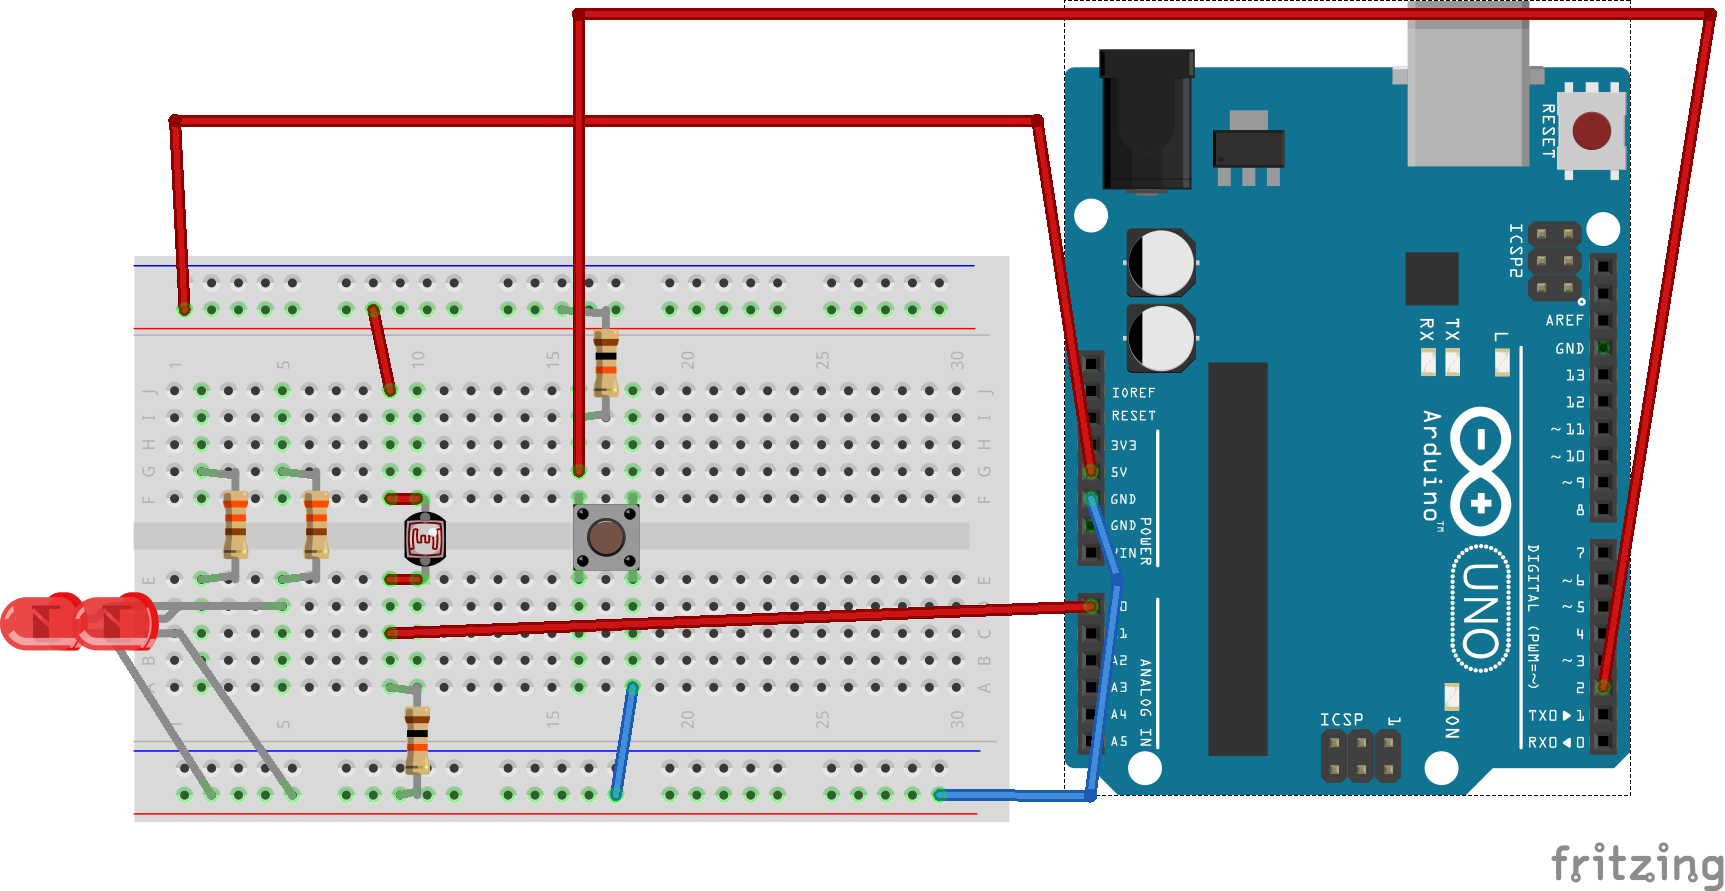
\includegraphics[width=7.0cm]{images/bread.png}
\caption{基礎実験4で使用した回路の配線図}
\label{fig:bread}
\end{center}
\end{figure}

\section{タイマ割り込みによるLEDの点滅}
課題2.4.1において作成したスケッチおよび完成させた図2.63を報告せよ.また,MsTimer2を使用せずにポーリング処理のみを使用した場合どのような問題点があるのか調査し,報告せよ.

以下ソースコード\ref{code:kadai2-4-1}に作成したスケッチを示す.

\begin{lstlisting}[caption = 課題2.4.1,label=code:kadai2-4-1][H]
#include <MsTimer2.h>
const int LED1_PIN = 13; //13番ピンにLEDを接続
const int LED2_PIN = 9; //9番ピンにLEDを接続

void flash() { //割り込みサービスルーチン(LEDの点滅)
  for ( int i = 255; i >= 0 ; i--){ //発光状態から消灯状態へ
    analogWrite(LED2_PIN,i); //LED2_PINにPWM出力
    delay(5000/256); //256回(発光->消灯間5000ms)
  }
  
}

void setup() {
  pinMode(LED1_PIN, OUTPUT); //13番ピンを出力ポートに設定
  pinMode(LED2_PIN,OUTPUT); //9番ピンを出力ポートに設定
  MsTimer2::set(20, flash); // タイマ割り込み間隔の設定(500ms)
  MsTimer2::start(); //タイマ割り込み開始
}

void loop() { //ボーリング処理
  digitalWrite(LED1_PIN,HIGH); //13番ピンに5V出力
  delay(500); //500ms待機
  digitalWrite(LED1_PIN,LOW); //13番ピンに0V出力
  delay(500); //500ms待機
}
\end{lstlisting}

また,以下図\ref{fig:2-63}に完成させた図2.63を示す.

\begin{center}

\includegraphics[width=7.0cm]{images/figure2-63.png}
\caption{ポーリングと割り込みによる周期の異なるLEDの同時点滅}
\label{fig:2-63}
\end{center}
\end{figure}

MsTimer2を使用せずにポーリング処理のみを使用した場合は,

//~~~~ここを書く~~~~~~


\section{タイマ割り込みによる照度センサのデータ取得}
課題2.4.2において作成したスケッチを報告せよ.また,「手で光を遮る」「光を遮らない」状態を素早く繰り返した時に生じた取りこぼしについて原因を考察せよ.さらに,取りこぼしを回避する方法案を記せ.

以下ソースコード\ref{code:kadai2-4-2}に作成したスケッチを示す.


\begin{lstlisting}[caption = 課題2.4.2,label=code:kadai2-4-2][H]
unsigned long timePrev = 0; //基準となる時間を格納

void check() {
  static int sensorvalue = analogRead(A0); //A0ピンのAD変換結果を取得
  Serial.println(sensorvalue);
}
void setup() {
  Serial.begin(9600); //シリアル通信を9600kbpsで初期化
  pinMode(13,OUTPUT); //13番ピンを出力ポートに設定
}

void loop() { //millis関数による時間計測
  unsigned long timeNow = millis(); //millis関数を用いて現在の時間情報を取得
  if(timeNow - timePrev >= 500){ //500ms以上経過
    check(); //check関数の処理を実行
    timePrev = timeNow; //時間情報の更新
  }
  else{}
}
\end{lstlisting}
「手で光を遮る」「光を遮らない」状態を素早く繰り返した時に生じた取りこぼした原因は,mills関数の値にある.500msごとにセンサの値を読み取っているため500msの間にあった変化に関してはセンサは読み込めない.取りこぼしを回避するにはmills関数の値をより小さくして細かくセンサの値を読み取る必要があるが,細かくしすぎると値を読み取る回数が増えて処理が重くなる.

\section{スイッチ動作の外部割り込みによるLEDの点灯・消灯}
演習2.4.5において生じるチャタリングについて調査し報告せよ.また,attachInterruptを使用せずにポーリング処理のみを使用した場合,どのような問題が生じるのか調査し,報告せよ.

チャタリングとは,物理的なスイッチなどを使用した時,スイッチを押した瞬間にONとOFFの状態が非常に短い間隔で振動することである.今回の実験では物理スイッチを用いているため,ONにした瞬間にONとOFFが交互に動作して誤動作を起こしている.\\
また,attachInterruptを使用せずにポーリング処理のみを使用した場合,ループ関数の中で処理を定義する必要がある.ループ関数で処理を行っている途中に外部割り込みがあった場合,外部割り込みを認識できないか,反応が遅れる..またループ処理の中で信号を検知する場合,常に信号があるかないかを確認する必要があるので処理が多くなる.
\section{スイッチ動作に外部割り込みによるLED発行のフェイドイン・フェイドアウト}
課題2.4.3で作成したスケッチを報告せよ.またスケッチで工夫した点を工夫せよ.

以下ソースコード\ref{code:kadai2-4-3}に作成したスケッチを示す.

\begin{lstlisting}[caption = 課題2.4.3,label=code:kadai2-4-3][H]

\end{lstlisting}

スケッチで工夫した点は

//~~~~ここを書く~~~~~

\section{発展課題2.4.1}
発展課題2.4.1において作成したスケッチと工夫点を報告せよ.また,照度センサの値の変化をグラフ化し,その結果を報告せよ.

以下ソースコード\ref{code:hatten2-4-1}に作成したスケッチを示す.

\begin{lstlisting}[caption = 発展課題2.4.1,label=code:hatten2-4-1][H]

\end{lstlisting}

スケッチで工夫した点は,

また以下図\ref{fig:hatten2-4-1}に照度センサの値の変化のグラフを示す.

\begin{center}
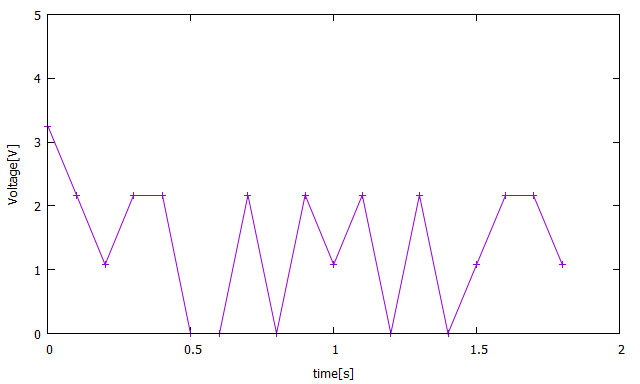
\includegraphics[width=7.0cm]{images/hatten2-4-1.png}
\caption{照度センサの値の変化}
\label{fig:hatten2-4-1}
\end{center}
\end{figure}



\section{発展課題2.4.2}
発展課題2.4.2において作成したスケッチと工夫点を報告せよ.また,照度センサの値の変化をグラフ化し,その結果を報告せよ.

以下ソースコード\ref{code:hatten2-4-2}に作成したスケッチを示す.

\begin{lstlisting}[caption = 発展課題2.4.2,label=code:hatten2-4-2][H]

\end{lstlisting}

スケッチで工夫した点は,

また以下図\ref{fig:hatten2-4-1}に照度センサの値の変化のグラフを示す.

\begin{center}
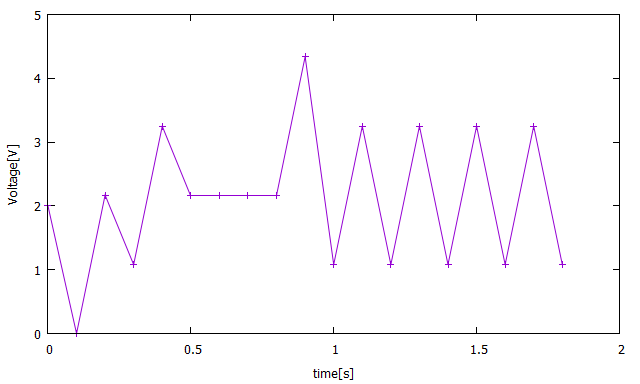
\includegraphics[width=7.0cm]{images/hatten2-4-2.png}
\caption{照度センサの値の変化}
\label{fig:hatten2-4-2}
\end{center}
\end{figure}

\section{発展課題2.4.3}
発展課題2.4.3において作成したスケッチと工夫点を報告せよ.

以下ソースコード\ref{code:hatten2-4-3}に作成したスケッチを示す.

\begin{lstlisting}[caption = 発展課題2.4.3,label=code:hatten2-4-3][H]

\end{lstlisting}

スケッチで工夫した点は,

\end{document}
